\section{System}
\label{sec:sys}

\begin{figure}[t]
\centering
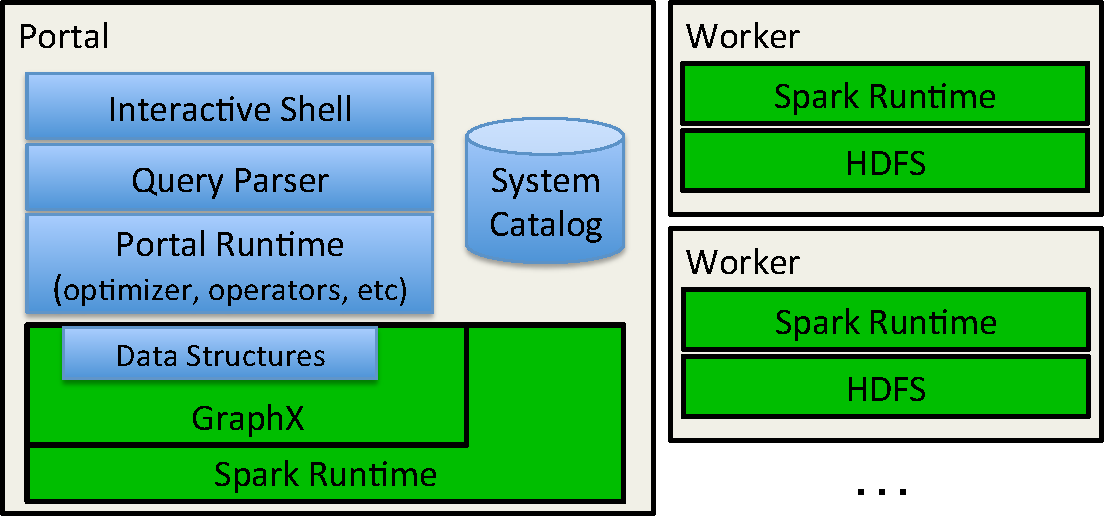
\includegraphics[width=3.4in]{figs/architecture.pdf}
\vspace{-0.4cm}
\caption{\sys system architecture.}
\vspace{-0.4cm}
\label{fig:arch}
\end{figure}

We developed a prototype system \sys that is implemented on top of
Apache Spark/GraphX~\cite{DBLP:conf/osdi/GonzalezXDCFS14}/Spark SQL,
as depicted in Figure~\ref{fig:arch}.  Green boxes indicate built-in
components, while blue are those we added for \sys.  Data is
distributed in partitions across the cluster workers, is read in from
the distributed file system (HDFS), and can be viewed both as a graph
and as a pair of RDDs.  All \tg operations are available through the
public API of the \sys library, and may be used in an Apache Spark
application.

{\bf Temporal operators.}  Apache Spark is not a temporal DBMS but
rather an open-source in-memory distributed framework that combines
graph-parallel and data-parallel abstractions.  We reduce our temporal
operators into a sequence of non-temporal relational operators or their
equivalents for Spark RDDs, maintaining point semantics.  In some
cases, such as temporal window node creation, access methods based on
GraphX graphs provide significantly more efficient performance.  For
analytics, we use the GraphX Pregel library, but add a batching method
to compute overall time instances together,
see~\cite{MoffittTempWeb16} for a detailed discussion.\eat{ \sys
  supports PageRank, connected components, and shortest paths
  analytics out of the box, and provides an API for adding others.  We
  are in the process of adding the clustering coefficient analytic.}

{\bf Query evaluation.}  \sys query execution follows the traditional
query processing steps: parsing, logical plan generation and
verification, and physical plan generation. \sys re-uses and extends
SparkSQL abstractions for these steps.  A \ql query is rewritten into
a sequence of \tga operators, and some operators are reordered in a
rule-based manner to improve performance. \julia{How do we rewrite
  \tga into \tra then?  In what way to we use SparkSQL?  This part
  needs to be explained.}

\julia{Need a paragarph here about rule-based query optimziation in
  \tga.}

\eat{For example, pushing slice improves performance similar to
  pushing selection in SQL.}

\eat{For example, pushing temporal aggregation
  before temporal join can sometimes lead to better performance. A
  temporal join query may be rewritten to include additional temporal
  selection conditions, based on information about the temporal schema
  of the TGraphs being joined, which in turn significantly reduces
  data load time.}

We developed several physical representations and partitioning
strategies that are selected at the physical plan generation
stage. \tgs are read into memory from HDFS and processed by Spark
Workers, with task assignment managed by the runtime.  Details about
the physical representations can be found in~\cite{PortalarXiv2016}.

\begin{figure}[t]
\centering
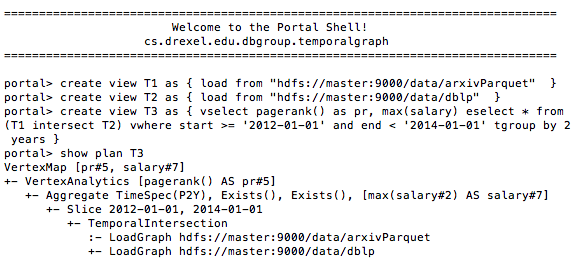
\includegraphics[width=3.4in]{figs/shell.png}
\caption{\sys interactive shell.}
\label{fig:shell}
\end{figure}

{\bf Interactive shell. Integration with SQL.}  The \sys system
includes an interactive shell for exploratory data analysis
(Figure~\ref{fig:shell}). Shell users can execute queries, define
(materialized) views, inspect query execution plans, and execute SQL
queries with an embedded \ql view. Consider the following SQL query
that returns \insql{vid} and \insql{tr} values of 20 vertices with the
most significantly increasing PageRank trend.

\begin{small}
\begin{verbatim}
Select VF.vid, VF.tr
From T5.vertices() as VF
Order by tr
Limit 20
\end{verbatim}
\end{small}

An important part of the query is the use of \insql{T5.vertices()} in
the \insql{From} clause. This is an operation provided by the \sys
framework, which takes as input all vertices of \insql{T5} and their
attributes in a single nested relation \insql{VF}, with schema
\insql{(vid:long, start:date, end:date, tr:float)}. \insql{VF} can be
used in SQL queries. \sys also provides an operation \insql{edges()}
that returns a similar relation for the edges of a given \tg.



